\section{Auswertung}
\label{sec:auswertung}
Im Folgenden werden alle Fehler mit Hilfe der \texttt{python}-Bibliothek
\texttt{uncertainties}\cite{py-uncertainties} berechnet, die eine Gaußsche
Fehlerfortpflanzung implementiert.

\subsection{Frequenzgang eines gegenkekoppelten Verstärkers} % (fold)

Im folgenden wird der Frequenzgang eines gegengekoppelten Verstärkers bei vier verschiedenen Verstärkungsgraden $V'$.
Dazu wurde die Schaltung \ref{} verwendet.
Bei allen Messungen wurde eine Eingangsspannung von $\SI{15}{\milli\ohm}$ verwendet.
Zudem ist auf den Widerstand $R_1$ noch der Innenwiderstand der Spannungsquelle mit $R_i = \SI{50}{\ohm}$ aufaddiert worden.

\paragraph{Verstärungsgrad 1 $\frac{\SI{1}{\mega\ohm}}{\SI{100}{\ohm}}$}

\begin{table}
\centering
\caption{Messwerte zum Verstärkungsgrad 1.}
    \label{tab:a_messwerte_1}
    \input{build/a_data_1.tex}
\end{table}

In Grafik \ref{fig:a_plot_1} sind die gemessenen Messdaten aus Tabelle \ref{tab:a_messwerte_1} halblogarithmisch dargestellt.
Mithilfe einer linearen Regression der Form $f_1(x)= m \cdot x + b$ wird die Steigung der fallenden Geraden bestimmt.
Es ergibt sich
\begin{equation*}
	f_{a,1}(x) = (\num{-0.9480(1)}) \cdot x + (\num{13.0129(111)})\,.
\end{equation*}
Die Grenzfrequenz $\nu'_{g,1}$ - die Frequenz, bei der die Verstärkung auf $\frac{V'_1}{\sqrt{2}}$ abgefallen ist - kann bei dieser Verstärkung nicht bestimmt werden, da kein Plateau bei geringen Frequenzen erkennbar ist.
Somit kann auch keine Leerlaufverstärkung $V_1$ abgeschätzt werden.

\begin{figure}[h!]
    \centering
    \includegraphics[width=0.8\linewidth]{build/a_plot_1.pdf}
    \caption{Frequenzgang eine gegengekoppelten Verstärkers mit einer Verstärkung von $10\,\mathrm{k}$.}
    \label{fig:a_plot_1}
\end{figure}

\paragraph{Verstärungsgrad 2 $\frac{\SI{120}{\kilo\ohm}}{\SI{100}{\ohm}}$}

\begin{table}
\centering
\caption{Messwerte zum Verstärkungsgrad 2.}
    \label{tab:a_messwerte_2}
    \input{build/a_data_2.tex}
\end{table}

In Grafik \ref{fig:a_plot_2} sind die gemessenen Messdaten aus Tabelle \ref{a_tab_2} halblogarithmisch dargestellt.
Mithilfe einer linearen Regression der Form $f_2(x)= m \cdot x + b$ wird die Steigung der fallenden Geraden bestimmt.
Es ergibt sich
\begin{equation*}
	f_{a,2}(x) = (\num{-0.9652(2)}) \cdot x + (\num{13.0827(191)})\,.
\end{equation*}
Die Grenzfrequenz $\nu'_{g,2}$ - die Frequenz, bei der die Verstärkung auf $\frac{V'_2}{\sqrt{2}}$ abgefallen ist - ist zu $\nu'_{g,2} = \SI{1567.4(193)}{\hertz}$ bestimmt worden.
Der Wert für die Verstärkung $V'_2$ lässt sich aus dem Wert des Plateaus zu $V'=560.0\pm6.7$ bestimmen.
Die ideale Verstärkung 
\begin{equation*}
    V'_{2,\text{ideal}} = \frac{R_N}{R_1} \approx 800.0
\end{equation*}
weicht somit um etwa $\SI{30}{\percent}$ von der gemessenen ab.
Mithilfe der Gleichung \eqref{calc_V} wird die Leerlaufverstärkung $V_2$ zu
\begin{equation*}
	V_2 = \frac{1}{V'_2} - \frac{R_1}{R_N} = \frac{1}{560.0\pm6.7} - \frac{\SI{150}{\ohm}}{\SI{120}{\kilo\ohm}} \approx 
    \num{1.87(7)e3}
\end{equation*}

\begin{figure}[h!]
    \centering
    \includegraphics[width=0.8\linewidth]{build/a_plot_2.pdf}
    \caption{Frequenzgang eine gegengekoppelten Verstärkers mit einer Verstärkung von $1200$.}
    \label{fig:a_plot_2}
\end{figure}

\paragraph{Verstärungsgrad 3 $\frac{\SI{4.7}{\kilo\ohm}}{\SI{100}{\ohm}}$}

\begin{table}
\centering
\caption{Messwerte zum Verstärkungsgrad 3.}
    \label{tab:a_messwerte_3}
    \input{build/a_data_3.tex}
\end{table}

In Grafik \ref{fig:a_plot_3} sind die gemessenen Messdaten aus Tabelle \ref{a_tab_3} halblogarithmisch dargestellt.
Mithilfe einer linearen Regression der Form $f_3(x)= m \cdot x + b$ wird die Steigung der fallenden Geraden bestimmt.
Es ergibt sich
\begin{equation*}
    f_{a,3}(x) = (\num{-0.7991(1)}) \cdot x + (\num{11.0282(187)})\,.
\end{equation*}
Die Grenzfrequenz $\nu'_{g,3}$ - die Frequenz, bei der die Verstärkung auf $\frac{V'_3}{\sqrt{3}}$ abgefallen ist - ist zu $\nu'_{g,3} = \SI{3.060(6)e4}{\hertz}$ bestimmt worden.
Der Wert für die Verstärkung $V'_3$ lässt sich aus dem Wert des Plateaus zu $V'=22.667\pm0.033$ bestimmen.
Die ideale Verstärkung 
\begin{equation*}
    V'_{3,\text{ideal}} = \frac{R_N}{R_1} \approx 31.33
\end{equation*}
weicht somit um etwa $\SI{27}{\percent}$ von der gemessenen ab.
Mithilfe der Gleichung \eqref{calc_V} wird die Leerlaufverstärkung $V_3$ zu
\begin{equation*}
    V_3 = \frac{1}{V'_3} - \frac{R_1}{R_N} = \frac{1}{22.667\pm0.033} - \frac{\SI{150}{\ohm}}{\SI{4.7}{\kilo\ohm}} \approx \num{81.9\pm0.4}
\end{equation*}

\begin{figure}[h!]
    \centering
    \includegraphics[width=0.8\linewidth]{build/a_plot_3.pdf}
    \caption{Frequenzgang eine gegengekoppelten Verstärkers mit einer Verstärkung von $47$.}
    \label{fig:a_plot_3}
\end{figure}

\paragraph{Verstärungsgrad 4 $\frac{\SI{1}{\mega\ohm}}{\SI{4.7}{\kilo\ohm}}$}

\begin{table}
\centering
\caption{Messwerte zum Verstärkungsgrad 4.}
    \label{tab:a_messwerte_4}
    \input{build/a_data_4.tex}
\end{table}

In Grafik \ref{fig:a_plot_4} sind die gemessenen Messdaten aus Tabelle \ref{a_tab_4} halblogarithmisch dargestellt.
Mithilfe einer linearen Regression der Form $f_4(x)= m \cdot x + b$ wird die Steigung der fallenden Geraden bestimmt.
Es ergibt sich
\begin{equation*}
    f_{a,4}(x) = (\num{-0.8821(2)}) \cdot x + (\num{12.1148(217)})\,.
\end{equation*}
Die Grenzfrequenz $\nu'_{g,4}$ - die Frequenz, bei der die Verstärkung auf $\frac{V'_4}{\sqrt{4}}$ abgefallen ist - ist zu $\nu'_{g,4} = \SI{4.57(11)e3}{\hertz}$ bestimmt worden.
Der Wert für die Verstärkung $V'$ lässt sich aus dem Wert des Plateaus zu $V'_4=152.7\pm3.3$ bestimmen.
Die ideale Verstärkung 
\begin{equation*}
    V'_{4,\text{ideal}} = \frac{R_N}{R_1} \approx 210.53
\end{equation*}
weicht somit um etwa $\SI{27}{\percent}$ von der gemessenen ab.
Mithilfe der Gleichung \eqref{calc_V} wird die Leerlaufverstärkung $V_4$ zu
\begin{equation*}
    V_4 = \frac{1}{V'_4} - \frac{R_1}{R_N} = \frac{1}{152.7\pm3.3} - \frac{\SI{4.75}{\kilo\ohm}}{\SI{1}{\mega\ohm}} \approx \num{560\pm40}
\end{equation*}

\begin{figure}[h!]
    \centering
    \includegraphics[width=0.8\linewidth]{build/a_plot_4.pdf}
    \caption{Frequenzgang eine gegengekoppelten Verstärkers mit einer Verstärkungsgrad von $212.77$.}
    \label{fig:a_plot_4}
\end{figure}

\paragraph{Grenzfrequenz - Verstärkungsgrad Produkt}

Es wurde die Schaltung \ref{} verwendet.
Die Ergebnisse für das Produkt aus Grenzfrequenz $\nu'_{g,i}$ und Verstärkung $V'_i$ sind in Tabelle \ref{tab:a_nu_v} aufgerführt.
\begin{table}[h!]
\centering
\caption{Produkt aus Grenzfrequenz $\nu'_{g,i}$ und Verstärkung $V'_i$ der Messaufbauten 2 bis 4.}
    \label{tab:a_nu_v}
    \begin{tabular}{S[table-format=3.3(3)] S[table-format=3.3(2)] S[table-format=1.4(2)]}
            \toprule
            {Grenzfrequenz $\nu'_{g,i}/\si{\hertz}$} & {Verstärkung $V'_i$} & {$V'_i\cdot\nu'_{g,i}/\SI{e5}{\hertz}$}\\
            \midrule
            1567.4(193) & 560.0(67)  & 8.8032(20) \\
            30600(60)  & 22.667(33) & 6.9354(26)    \\
            4570(110)  & 152.7(33)  & 6.973(20)    \\
            \bottomrule
    \end{tabular}    
\end{table}
Es ist zu erkennen, dass die Größenordnung des Produktes dieselbe ist und die Werte maximal um etwa $\SI{20}{\percent}$ voneinander abweichen.

\subsection{Klemmenspannung eines speziellen NF-Generators}
\label{sub:klemmenspannung_eines_speziellen_nf_generators}

In den Schaltungen \ref{} und \ref{} wurden die Widerstände $R_N = \SI{12}{\kilo\ohm}$ und $R_1 = \SI{100}{\ohm}$ gewählt.
Die Ergebnisse der Ausgangsspannungen sind in Tabelle \ref{tab:b_volt}
Der Unterschied in der Ausgangsspannung könnte sich durch die verschiedenen Eingangswiderstände der Schaltungen erklären lassen.

\begin{table}[h!]
    \centering
    \caption{Vergleich der Klemmenspannung eines speziellen NF-Generators mithilfe einer gegengekoppelten und einer Elektrometer-Verstärkerschaltung mit etwa der gleichen Verstärkung $V'$.}
    \label{tab:b_volt}
    \begin{tabular}{S[table-format=3.0] S[table-format=1.1(1)] S[table-format=2.1(1)]}
        \toprule
        {$\nu/\si{\hertz}$} & {$U_\mathrm{Gg}/\si{\volt}$} & {$U_\mathrm{Elek}/\si{\volt}$}\\
        \midrule
         50 & 8.4(1) & 12.5(1) \\
        100 & 8.4(1) & 12.5(1) \\
        150 & 8.4(1) & 12.3(1) \\
        200 & 8.3(1) & 12.1(1) \\
        250 & 8.3(1) & 11.9(1) \\
        \bottomrule
    \end{tabular}
\end{table}

\subsection{Messung des Eingangswiderstandes $R_e$ und der Leerlaufverstärkung $V$} % (fold)
\label{sub:}

Für die Berechnung des Eingangswiderstandes wurde die Schaltung \ref{} verwendet und für die Generatorspannung $U_g = \SI{1.0(1)}{\volt}$, den Generatorwiderstand $R_v = \SI{10}{\kilo\ohm}$ und den Widerstand $R_N = \SI{100}{\kilo\ohm}$ gewählt.
Die Ergebnisse sind in Tabelle \ref{tab:c_ergebnisse} aufgeführt. Das Ergebnis in dem Frequenzbereich von $\SIrange{100}{1600}{\hertz}$ ist in der doppellogarithmischen Grafik \ref{fig:c_plot} dargestellt. Zudem ist in der doppellogarithmischen Grafik \ref{fig:c_plot_full} der Frequenzbereiches von $\SIrange{100}{100000}{\hertz}$ abgebildet.

Mithilfe der Gleichung
\begin{equation*}
    I = \frac{U_g}{R_v}
\end{equation*}
berechnet sich $I = \input{build/c_I.tex}$.
Mithilfe von $I$ ergibt sich nun der Eingangswiderstand $R_e$ aus dem Zusammenhang
\begin{equation*}
    R_e = \frac{U_e}{I}\,.
\end{equation*}
$U_a$ berechnet sich somit zu
\begin{equation*}
    U_a = R_N \cdot I = \input{c_U_a.tex} \,.
\end{equation*}
Die Ergebnis der Messung bis $\SI{20}{\kilo\hertz}$ liegen somit innerhalb des Fehlers des berechneten Wertes.
Die Leerlaufverstärkung $V$ lässt sich mithilfe von 
\begin{equation*}
    V = \frac{R_N}{R_e}
\end{equation*}
berechnen.

Mithilfe einer linearen Regression der Form $f_{c,R}(x) = m \cdot x + b$ ergeben sich für die linearen Bereiche die Geradengleichungen 
\begin{eqnarray*}
    f_{c,R,1}(x) &=& (\num{1.0452}) \cdot x + (\num{-3.4633(24)}) \,, \\
    f_{c,V,1}(x) &=& (\num{-1.0452}) \cdot x + (\num{14.9763(24)}) \,, \\
    f_{c,R,2}(x) &=& (\num{1.0493(1)}) \cdot x + (\num{-3.495(5)}) \,, \\
    f_{c,V,2}(x) &=& (\num{-1.0493(1)}) \cdot x + ( ) \,.
\end{eqnarray*}
Da die Steigungen im Bereich kleiner Freqeunzen bis auf die dritte Nachkommastelle mit denen größerer Frequenzen übereinstimmt, bestimmt sich der Frequenzbereich, in dem der Operationsverstärker einwandfrei arbeitet, zu $\SIrange{100}{20000}{\hertz}$.
Somit ist die Grenzfrequenz $\nu_g \approx \SI{20}{\kilo\hertz}$.
In den Messwerten ist dies gerade durch den Wert für die Frequenz $\nu$ erkennbar, an dem die Ausgangsspannung $U_a$ aufhört konstant zu bleiben.
Dies ist somit auch der Bereich, indem nicht mehr $R_v \gg R_e$ gilt und somit auch der Strom $I$ nicht mehr als konstant angenommen werden darf.

\begin{figure}[h!]
    \centering
    \includegraphics[width=0.8\linewidth]{build/c_plot.pdf}
    \caption{Doppellogarithmische Darstellung des Widerstands $R_e$ und der Leerlaufverstärkung $V$ in Abhängigkeit der Frequenz $\nu$ im Bereich $\SIrange{100}{1600}{\hertz}$.}
    \label{fig:c_plot}
\end{figure}

\begin{figure}[h!]
    \centering
    \includegraphics[width=0.8\linewidth]{build/c_plot_full.pdf}
    \caption{Doppellogarithmische Darstellung des Widerstands $R_e$ und der Leerlaufverstärkung $V$ in Abhängigkeit der Frequenz $\nu$ im Bereich $\SIrange{100}{100000}{\hertz}$.}
    \label{fig:c_plot_full}
\end{figure}

\begin{table}[h!]
    \centering
    \caption{Ergebnisse für den Eingangswiderstand $R_e$, die Leerlaufverstärkung $V$, die Eingangsspannung $U_e$ und die Ausgangsspannung $U_a$ bei verschiedenen Frequenzen $\nu$.}
    \label{tab:c_ergebnisse}
    \input{build/c_table.tex}
\end{table}

\subsection{Umkehr-Integrator}
Zur Überprüfung der Beziehung $U_a \approx \frac{1}{\nu}$ wurde die Schaltung nach Abbildung \ref{} verwendet.
Die verwendeten Daten sind in Tabelle \ref{tab:d_int_table} aufgelistet und in der doppellogarithmischen Abbildung \ref{fig:d_int_fig} dargestellt.
Mithilfe einer linearen Regression der Form $f_{d}(x) = m \cdot x + b$ ergibt sich für den linearen Bereich die Geradengleichung
\begin{equation*}
    f_{d}(x) = (\num{-0.9059}) \cdot x + (\num{5.2428(10)})\,.
\end{equation*}
Damit weicht der Exponent um etwa $\SI{10}{\percent}$ von der Beziehung $\approx \SI{1}{\nu}$ ab.
Somit ist der Frequenzbereich, in dem der Umkehr-Integrator arbeitet, $\SIrange{10}{640}{\hertz}$.
In Abbildung \ref{fig:int_sinus} ist eine integrierte Sinus-, in Abbildung \ref{fig:int_rechteck} eine integrierte Rechteck- und in Abbildung \ref{fig:int_dreieck} eine integrierte Dreieckspannung dargestellt.

\begin{table}[!h]
    \centering
    \caption{Aufgenommene Ausgangsspannungen $U_a$ einer Sinusspannung in Abhängigkeit der Frequenz $\nu$ mit einem Umkehr-Integrator.}
    \label{tab:d_int_table}
    \begin{tabular}{S[table-format=3.0] S[table-format=2.2(2)]}
    \toprule 
        {$\nu/\si{\hertz}$} & {$U/\si{\volt}$} \\
    \midrule
         10 &   23.50(10)\\
         20 &   12.10(10)\\
         40 &    6.91(01)\\
         80 &    3.66(01)\\
        160 &    1.89(01)\\
        320 &    1.01(01)\\
        640 &    0.54(01)\\
    \bottomrule
    \end{tabular}
\end{table}

\begin{figure}[!h]
    \centering
    \includegraphics[width=0.8\linewidth]{build/d_plot.pdf}
    \caption{Doppellogarithmische Darstellung der Ausgangsspannung $U_a$ gegen die Frequenz $\nu$ einer Sinusspannung mit einem Umkehr-Integrator.}
    \label{fig:d_int_fig}
\end{figure}

\begin{figure}[!h]
    \centering
    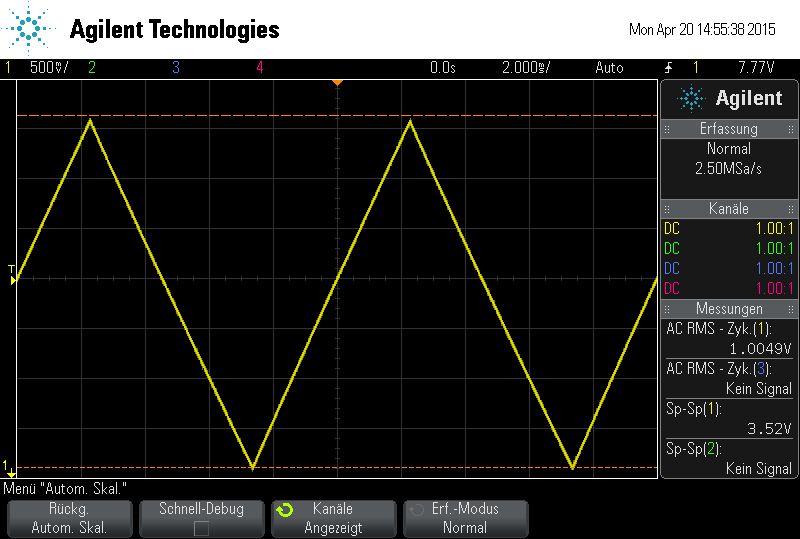
\includegraphics[width=0.8\linewidth]{data/scope_4.png}
    \caption{Integrierte Rechteckspannung.}
    \label{fig:int_rechteck}
\end{figure}

\begin{figure}[!h]
    \centering
    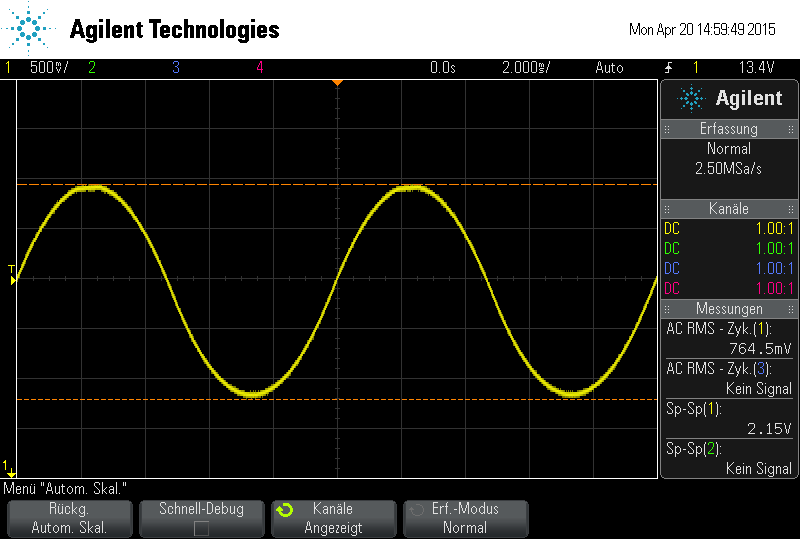
\includegraphics[width=0.8\linewidth]{data/scope_5.png}
    \caption{Integrierte Dreieckspannung.}
    \label{fig:int_dreieck}
\end{figure}

\begin{figure}[!h]
    \centering
    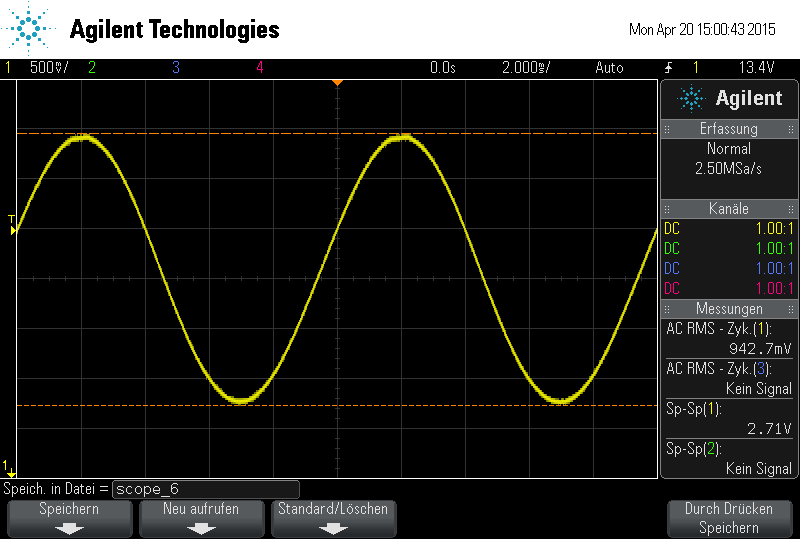
\includegraphics[width=0.8\linewidth]{data/scope_6.png}
    \caption{Integrierte Sinusspannung.}
    \label{fig:int_sinus}
\end{figure}

\subsection{Umkehr-Differentiator}
Es wurde ein Umkehr-Differentitor nach Schaltung \ref{} verwendet.
Die verwendeten Daten sind in Tabelle \ref{tab:e_dif_table} aufgelistet und in der doppellogarithmischen Abbildung \ref{fig:e_dif_fig} dargestellt.
Mithilfe einer linearen Regression der Form $f_{e}(x) = m \cdot x + b$ ergibt sich für den linearen Bereich die Geradengleichung
\begin{equation*}
    f_{e}(x) = (\num{0.967}) \cdot x + (\num{-7.705(8)})\,.
\end{equation*}
Der Frequenzbereich, in dem der Umkehr-Differentiator arbeitet, ist somit etwa $\SIrange{100}{6400}{\hertz}$.
In Abbildung \ref{fig:dif_sinus} ist eine differentierte Sinus-, in Abbildung \ref{fig:dif_rechteck} eine differentierte Rechteck- und in Abbildung \ref{fig:dif_dreieck} eine differentierte Dreieckspannung dargestellt.

\begin{table}[!h]
    \centering
    \caption{Aufgenommene Ausgangsspannungen $U_a$ einer Sinusspannung in Abhängigkeit der Frequenz $\nu$ mit einem Umkehr-Differentiator.}
    \label{tab:e_dif_table}
    \begin{tabular}{S[table-format=5.0] S[table-format=1.3(2)]}
    \toprule 
        {$\nu/\si{\hertz}$} & {$U/\si{\volt}$} \\
    \midrule
           10   0.012(01)
           20   0.015(01)
           40   0.023(01)
          100   0.041(01)
          200   0.076(01)
          400   0.143(01)
          800   0.272(01)
         1600   0.555(01)
         3200   1.100(10)
         6400   2.290(10)
        10000   4.220(10)
    \bottomrule
    \end{tabular}
\end{table}

\begin{figure}[!h]
    \centering
    \includegraphics[width=0.8\linewidth]{build/e_plot.pdf}
    \caption{Doppellogarithmische Darstellung der Ausgangsspannung $U_a$ gegen die Frequenz $\nu$ einer Sinusspannung mit einem Umkehr-Differentiator.}
    \label{fig:e_dif_fig}
\end{figure}


\begin{figure}[!h]
    \centering
    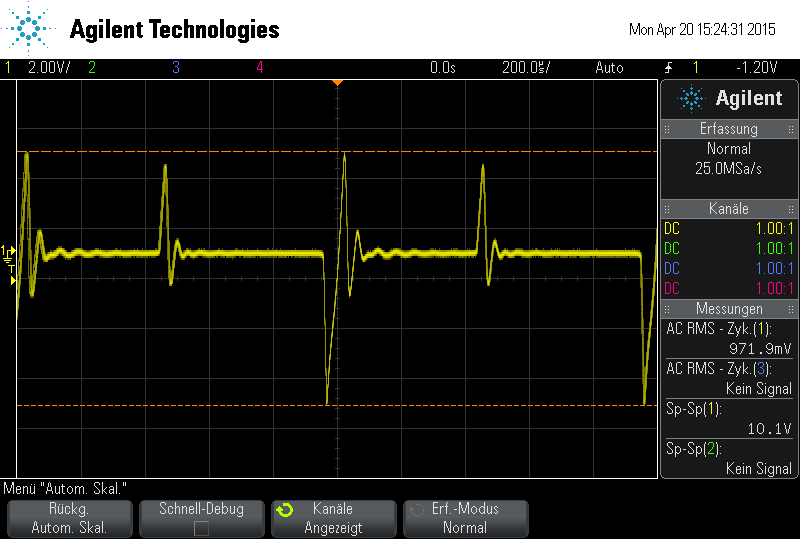
\includegraphics[width=0.8\linewidth]{data/scope_8.png}
    \caption{Differentierte Rechteckspannung.}
    \label{fig:dif_rechteck}
\end{figure}

\begin{figure}[!h]
    \centering
    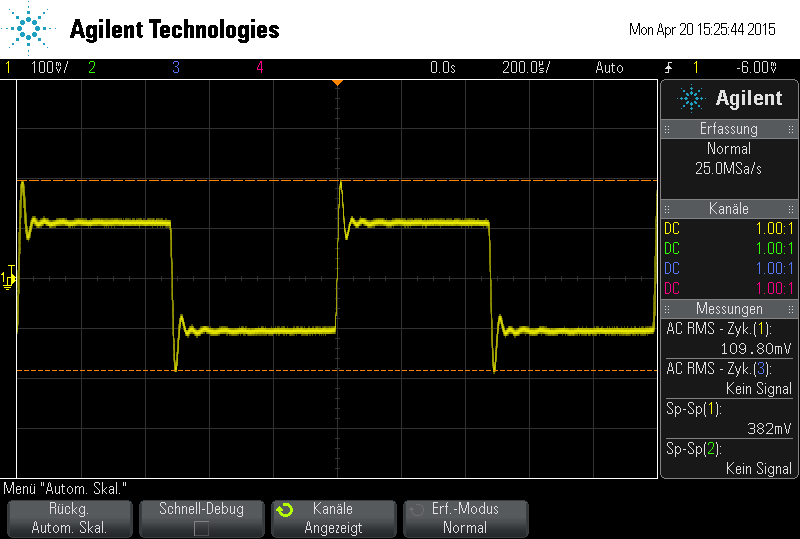
\includegraphics[width=0.8\linewidth]{data/scope_9.png}
    \caption{Differentierte Dreieckspannung.}
    \label{fig:dif_dreieck}
\end{figure}

\begin{figure}[!h]
    \centering
    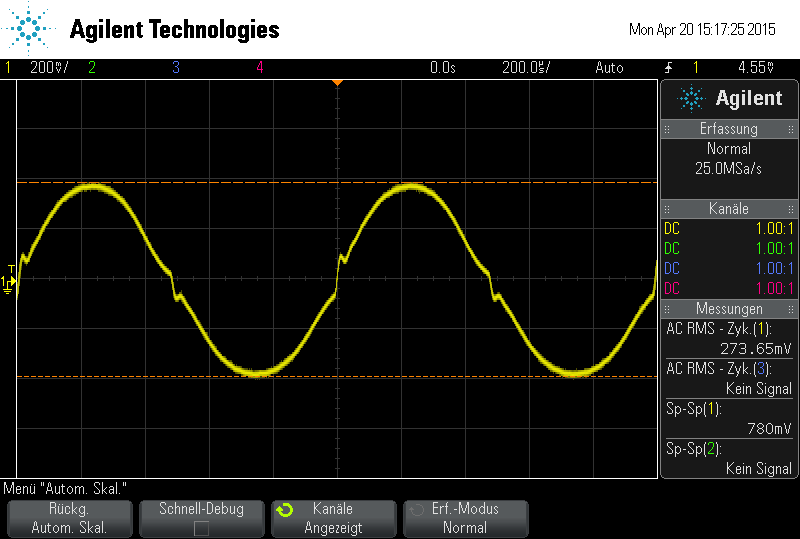
\includegraphics[width=0.8\linewidth]{data/scope_7.png}
    \caption{Differentierte Sinusspannung.}
    \label{fig:dif_sinus}
\end{figure}

\subsection{Schmitt-Trigger} % (fold)
\label{sub:schmitt_trigger}

Zur Bestimmung des Scheitelwertes eines Schmitt-Triggers wurde die Schaltung in Abbildung \ref{} verwendet.
Für die Schaltung wurden die Widerstände $R_1 = \SI{100}{\ohm}$ und $R_P = \SI{4.7}{\kilo\ohm}$ verwendet und der Zusammenhang $2 \cdot U_B = \SI{28.3}{\volt}$
Gemessen wurde dabei ein Umspringen des Schalters von dem in Abbildung \ref{fig:schmitt_offen} dargestellten Spannungsverlauf auf den in Abbildung \ref{fig:schmitt_geschlossen} dargstellten Spannungsverlauf bei $U_\text{kipp} \approx \SI{314}{\milli\volt}$.
Mithilfe der Gleichung
\begin{equation*}
    U_\text{kipp} = U_B \cdot \frac{R_1}{R_P} 
\end{equation*}
ergibt sich $U_\text{kipp} \approx \SI{301.06}{\milli\volt}$.
Dieser Wert weicht somit um etwa $\SI{4}{\percent}$ vom gemessenen Wert ab.

\begin{figure}[!h]
    \centering
    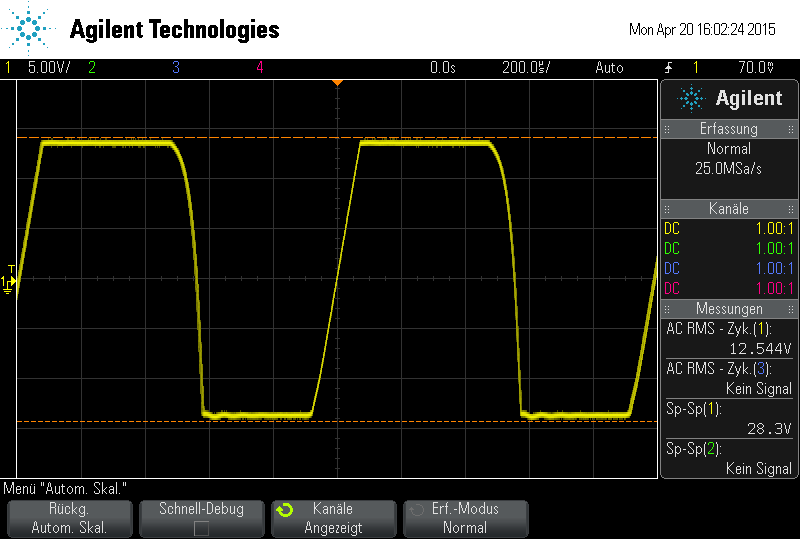
\includegraphics[width=0.8\linewidth]{data/scope_10.png}
    \caption{Schmitt-Trigger geöffnet.}
    \label{fig:schmitt_offen}
\end{figure}

\begin{figure}[!h]
    \centering
    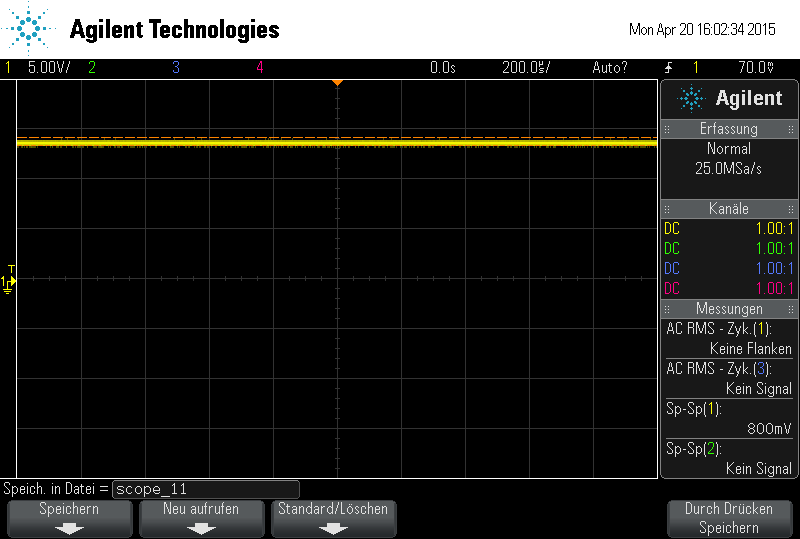
\includegraphics[width=0.8\linewidth]{data/scope_11.png}
    \caption{Schmitt-Trigger geschlossen.}
    \label{fig:schmitt_geschlossen}
\end{figure}

\subsection{Dreieckspannungsgenerator} % (fold)
\label{sub:dreiecksgenerator}

Mithilfe der Schaltung \ref{} wurde ein Dreieckspannungsgenerator realisiert.
Abbildung \ref{fig:rechteck} zeigt die zunächst generierte Rechteckspannung und Abbildung \ref{fig:dreieck} die finale Dreieckspannung.
Dabei wurde eine Frequenz von $\nu = \SI{1}{\kilo\hertz}$ und eine Spannung von $U_1 = \SI{200}{\milli\volt}$ gewählt.

\begin{figure}[!h]
    \centering
    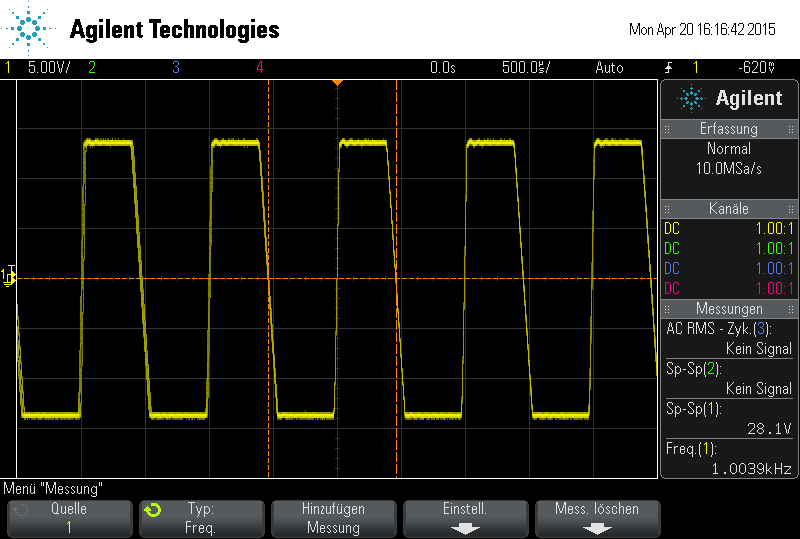
\includegraphics[width=0.8\linewidth]{data/scope_13.png}
    \caption{Generierte Rechteckspannung.}
    \label{fig:rechteck}
\end{figure}

\begin{figure}[!h]
    \centering
    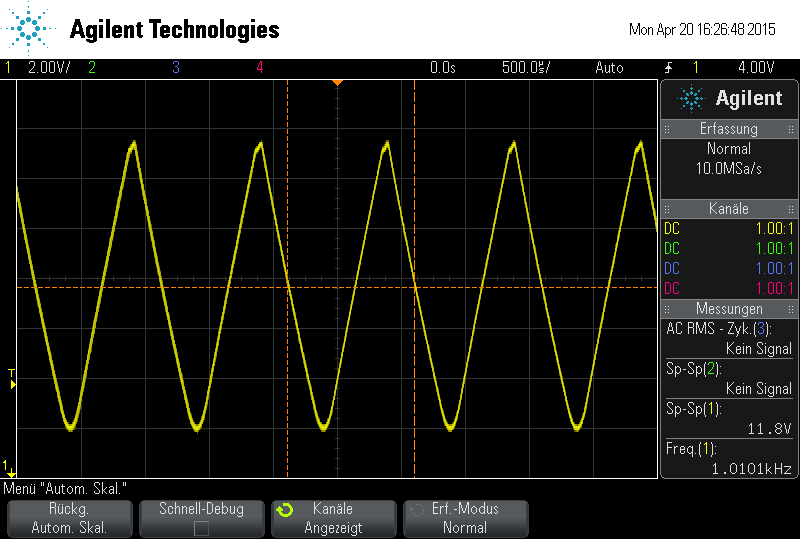
\includegraphics[width=0.8\linewidth]{data/scope_14.png}
    \caption{Generierte Dreieckspannung.}
    \label{fig:dreieck}
\end{figure}

\subsection{Gedämpfte Schwingung} % (fold)
\label{sub:subsection_name}

Zur realisierung einer gedämpften Schwingung wurde die Schaltung nach Abbildung \ref{} verwendet.
Für den Widerstand wurde $R = \SI{1}{\kilo\ohm}$ und für die Kapazität $C = \SI{20}{\nano\farad}$ gewählt.
Bei einer Dämpfungskonstante von $\eta = 0$ ergibt sich die in Abbildung \ref{fig:unged_sinus} dargestellte Schwingung.
Bei einer Dämpfungskonstante von $\eta = -1$ hingegen ergibt sich eine gedämpfte Schwingung wie in Abbildung \ref{fig:ged_sinus} dargestellt.
Die Amplituden der gedämpften Schwingung wurden der Grafik entnommen und sind in Tabelle \ref{tab:ged_schwing} aufgelistet.
Zudem sind die Daten in der halblogarithmischen Grafik \ref{fig:ged_schwing} dargestellt.
Mithilfe einer linearen Regression der Form $f_{d}(x) = x / \tau + b$ ergibt sich für den linearen Bereich die Geradengleichung
\begin{equation*}
    f_h(x) = \frac{x}{\num{-0.0046}} + (\num{-9.7(26)})\,.
\end{equation*}
Damit ergibt sich für die Abklingdauer $\tau \approx \num{-0.0046}$ und weicht somit von dem Theoriewert
\begin{equation*}
    \tau = 20 \cdot R \cdot C = 0.004
\end{equation*}
um etwa $\SI{15}{\percent}$ ab.

\begin{figure}[!h]
    \centering
    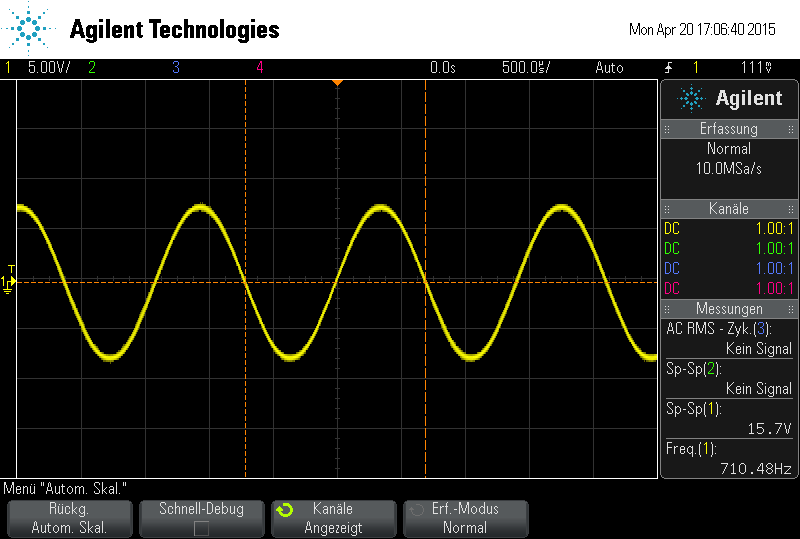
\includegraphics[width=0.8\linewidth]{data/scope_16.png}
    \caption{Ungedämpfte Sinusschwingung.}
    \label{fig:unged_sinus}
\end{figure}

\begin{figure}[!h]
    \centering
    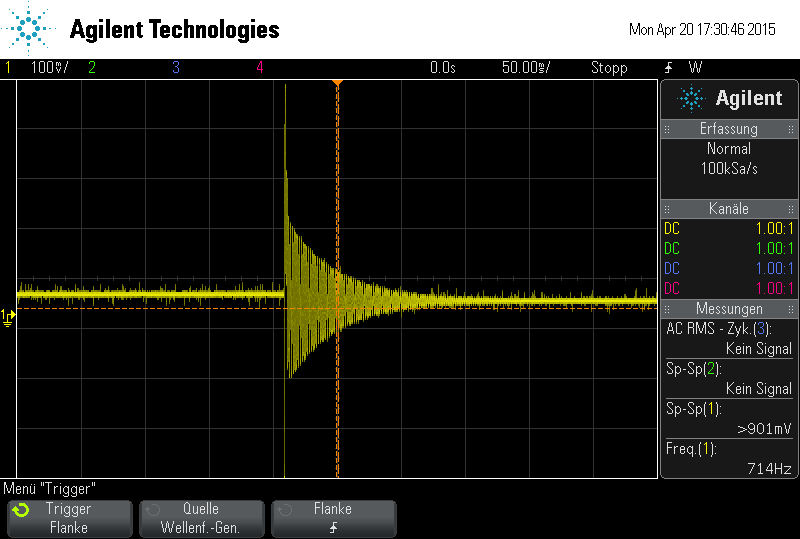
\includegraphics[width=0.8\linewidth]{data/scope_18.png}
    \caption{Gedämpfte Sinusschwingung.}
    \label{fig:ged_sinus}
\end{figure}

\begin{figure}[!h]
    \centering
    \includegraphics[width=0.8\linewidth]{build/h_plot.pdf}
    \caption{Amplituden der gedämpften Schwingung und lineare Regression zur Bestimmung der Abklingdauer $\tau$.}
    \label{fig:ged_schwing}
\end{figure}

\begin{table}[!h]
    \centering
    \caption{Gemessene Amplituden einer gedämpften Schwingung.}
    \label{tab:ged_schwing}
    \begin{tabular}
        \include{build/h_table.tex}
    \end{tabular}
\end{table}

\subsection{Logarithmierer} % (fold)
\label{sub:logarithmierer}

Für den logarithmierer wurde die Schaltung \ref{} verwendet.
Die aufgenommenen Daten sind in Tabelle \ref{tab:i_log} aufgelistet und in Grafik \ref{fig:i_log} halblogarithmisch dargestellt.
Mithilfe einer linearen Regression der Form $f_{d}(x) = m \cdot x + b$ ergibt sich für den linearen Bereich die Geradengleichung
\begin{equation*}
    f_{i}(x) = (\num{0.0480}) \cdot x + (\num{0.4303})\,.
\end{equation*}
Mithilfe der Beziehung
\begin{equation*}
    m = \frac{k_\mathrm{B} T}{e}\,,
\end{equation*}
wobei $k_\mathrm{B}$ die Boltzmann-Konstante, $T$ die Temperatur und $e$ die Elementarladung ist.
Damit ergibt sich die Temperatur zu $T \approx \SI{557}{\kelvin}$.
Die Änderung der Ausgangsspannung, wenn sich die Eingangsspannung um eine Zehnerpotenz ändert, bestimmt sich zu $\Delta U_a \approx \SI{108.3}{\milli\volt}$.

\begin{table}[!h]
    \centering
    \caption{Eingangsspannung $U_\text{ein}/\si{\volt}$ und Ausgangsspannung $U_\text{aus}/\si{\volt}$ eines logarithmierers.}
    \label{tab:i_log}
    \begin{tabular}{S[table-format=1.1] S[table-format=1.4(2)] S[table-format=2.1] S[table-format=1.4(2)]}
    \toprule 
        {$U_\text{ein}/\si{\volt}$} & {$U_\text{aus}/\si{\volt}$} & {$U_\text{ein}/\si{\volt}$} & {$U_\text{aus}/\si{\volt}$} \\
    \midrule
         0.0  &  0.2900(50)  &  6.5  &  0.5191(50) \\
         0.5  &  0.3956(50)  &  7.0  &  0.5234(50) \\
         1.0  &  0.4337(50)  &  7.5  &  0.5271(50) \\
         1.5  &  0.4505(50)  &  8.0  &  0.5307(50) \\
         2.0  &  0.4648(50)  &  8.5  &  0.5334(50) \\
         2.5  &  0.4752(50)  &  9.0  &  0.5364(50) \\
         3.0  &  0.4823(50)  &  9.5  &  0.5394(50) \\
         3.5  &  0.4897(50)  & 10.0  &  0.5420(50) \\
         4.0  &  0.4955(50)  & 11.0  &  0.5460(50) \\
         4.5  &  0.5005(50)  & 12.0  &  0.5503(50) \\
         5.0  &  0.5057(50)  & 13.0  &  0.5540(50) \\
         5.5  &  0.5105(50)  & 14.0  &  0.5574(50) \\
         6.0  &  0.5146(50)  & 15.0  &  0.5607(50) \\
    \bottomrule
    \end{tabular}
\end{table}

\begin{figure}[!h]
    \centering
    \includegraphics[width=0.8\linewidth]{build/i_log_plot.pdf}
    \caption{Halblogarithmische Darstellung der Ausgangsspannung $U_\text{aus}/\si{\volt}$ in Abhängigkeit von der Eingangsspannung $U_\text{ein}/\si{\volt}$ eines Logarithmierers.}
    \label{fig:i_log}
\end{figure}

\subsection{Exponentierer} % (fold)
\label{sub:Exponentierer}

Für den Exponentierer wurde die Schaltung \ref{} verwendet.
Die Ergebnisse sind in Tabelle \ref{tab:i_exp} aufgelistet und in Grafik \ref{fig:i_log} dargestellt.
Da in dem dargestellten Bereich kein exponentieller Zusammenhang 
erkennbar ist, ist eine Auswertung weiter nicht möglich.

\begin{table}[!h]
    \centering
    \caption{Eingangsspannung $U_\text{ein}/\si{\volt}$ und Ausgangsspannung $U_\text{aus}/\si{\volt}$ eines Exponentierers.}
    \label{tab:i_exp}
    \begin{tabular}{S[table-format=1.0] S[table-format=1.4(2)] S[table-format=2.0] S[table-format=2.4(2)]}
    \toprule 
        {$U_\text{ein}/\si{\volt}$} & {$U_\text{aus}/\si{\volt}$} & {$U_\text{ein}/\si{\volt}$} & {$U_\text{aus}/\si{\volt}$} \\
    \midrule
        0  &  -0.0336(10) & 8  &  -4.9490(10)
        1  &   2.0536(10) & 9  &  -6.0920(10)
        2  &   1.1365(10) & 10 &  -7.1390(10)
        3  &   0.3070(10) & 11 &  -8.2070(10)
        4  &  -0.6120(10) & 12 &  -9.2380(10)
        5  &  -1.7050(10) & 13 & -10.1440(10)
        6  &  -2.2788(10) & 14 & -10.9990(10)
        7  &  -3.7420(10) & 15 & -12.1130(10)
    \bottomrule
    \end{tabular}
\end{table}

\begin{figure}[!h]
    \centering
    \includegraphics[width=0.8\linewidth]{build/i_exp_plot.pdf}
    \caption{Darstellung der Ausgangsspannung $U_\text{aus}/\si{\volt}$ in Abhängigkeit von der Eingangsspannung $U_\text{ein}/\si{\volt}$ eines Exponentierers.}
    \label{fig:i_log}
\end{figure}

\subsection{Phasenabhängigkeit} % (fold)
\label{sub:phasenabhängigkeit}

Bei dem Verstärkungsgrad $V' = -\frac{\SI{120}{\kilo\ohm}}{\SI{100}{\ohm}} = -\num{1.2e3}$ ergiebt sich eine Phase von $\SI{180}{\degree}$.
Dies ist in Abbildung \ref{fig:phase_verlauf} als Spannungsverlauf der Eingangs- und Ausgangsspanung dargestellt und in Abbildung \ref{fig:lissa} in vorm einer Lissajou-Figur.

\begin{figure}[!h]
    \centering
    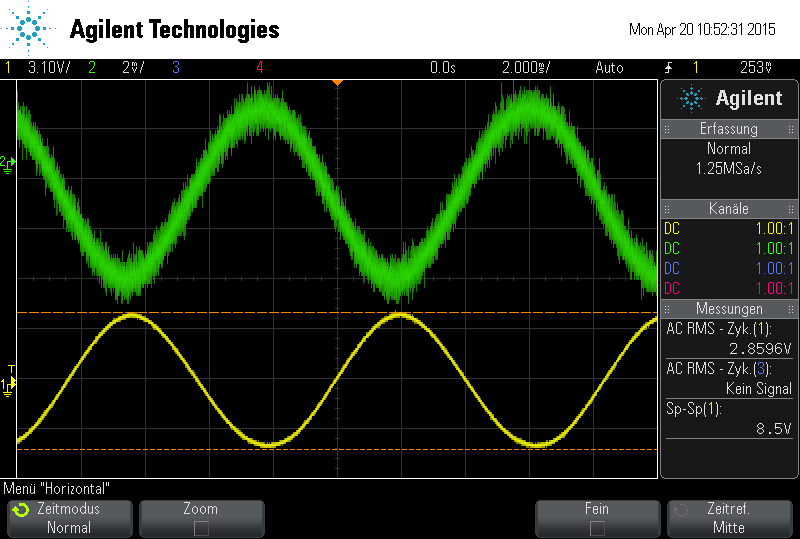
\includegraphics[width=0.8\linewidth]{data/scope_2.png}
    \caption{Darstellung der Ausgangsspannung und der Eingangsspannung.}
    \label{fig:phase_verlauf}
\end{figure}

\begin{figure}[!h]
    \centering
    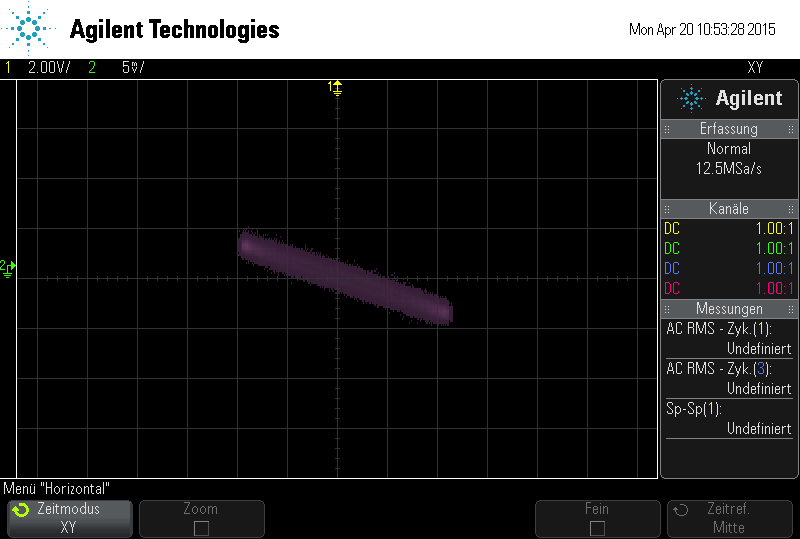
\includegraphics[width=0.8\linewidth]{data/scope_3.png}
    \caption{Darstellung der Phasenbeziehung der Ausgangsspannung und der Eingangsspannung als Lissajou Figur.}
    \label{fig:phase_liss}
\end{figure}